\chapter{Zeitauswertung}
Die Bachelorarbeit wird mit 12 ECTS Punkten honoriert. Pro ECTS Punkt wird mit einem Aufwand von ca. 30 Stunden gerechnet. Daraus ergibt sich für die Bachelorarbeit ein geplanter Zeitaufwand von 360 Stunden pro Teammitglied, also 720 Stunden Gesamtaufwand. Mit den erstellen Arbeitspaketen wurde ein Aufwand von 732 Stunden
geschätzt. Die Endabrechnung zeigt einen ungefähren Zeitaufwand von 842 Stunden. Daraus resultiert ein Gesamtaufwand von 421 Stunden pro Teammitglied. Die geforderten 360 Stunden pro Teammitglied wurden damit deutlich überschritten.

\begin{figure}[H]
\centering
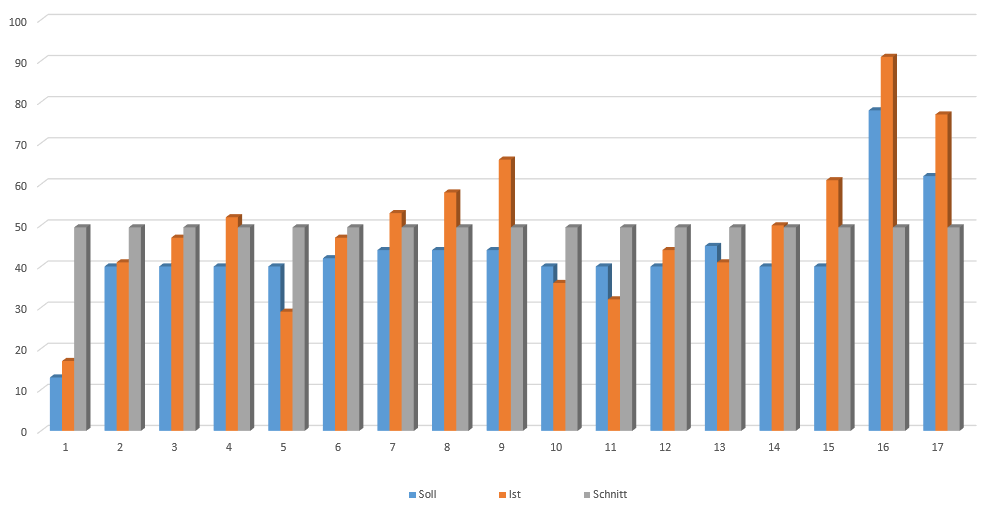
\includegraphics[width=1\textwidth]{../01_Projektplanung/images/weekly_done.png}
\caption{Arbeitsstunden wöchentlich}
\end{figure}

Die Zeitverteilung pro Kalenderwoche ist unterschiedlich. Die Aufwände im Programmierbereich waren oft deutlich höher als angenommen. In den Wochen 6-9 (Erstellung Prototyp) und 14-17 (Fertigstellung Software, Abschlussbericht) sind die Differenzen am höchsten. Dies ist einerseits mit teils geringen Vorkenntnissen, aber andererseits auch mit hohem Implementationsaufwand zu rechtfertigen. 

\begin{figure}[H]
\centering
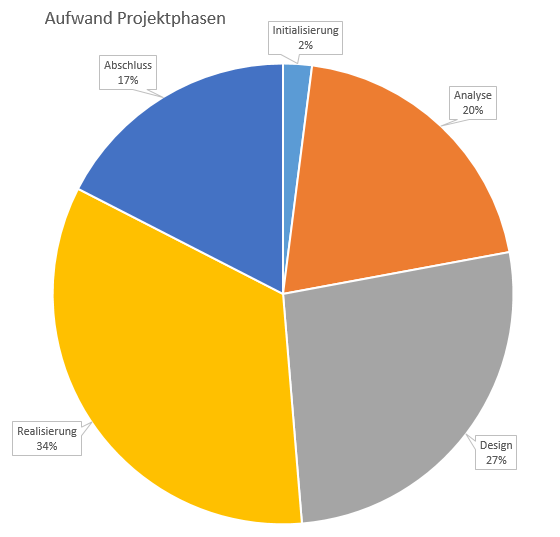
\includegraphics[width=0.6\textwidth]{../01_Projektplanung/images/aufwand_phasen.png}
\caption{Aufwände pro Projektphase}
\end{figure}

Durch die teils geringen Vorkenntnisse musste verhältnismässig viel Aufwand in Analyse und Prototyping gesteckt werden. $\frac{1}{3}$ Aufwand für die Realisierung scheint daher eher gering.